% !TEX program = xelatex
% ¡Recuerda compilar con XeLaTeX o LuaLaTeX!
\documentclass{article}

% --- Cargar nuestro fichero de estilo ---
% Se asume que paper_style.sty está disponible o se usan paquetes estándar.
\usepackage{paper_style}

% --- PAQUETES PARA EL CONTENIDO DEL DOCUMENTO ---
\usepackage{graphicx}
\usepackage{subcaption}
\usepackage{amsmath}
\usepackage{booktabs}
\usepackage{geometry}
\usepackage{hyperref}
\usepackage{enumitem}
\usepackage{float}
\usepackage{soul}
\usepackage{xcolor}


% --- Información del Paper ---
\title{Informe: \\ Práctica 3: Redes Virtuales y Seguridad de Acceso}
\author{
	Jordi Blasco Lozano \\
	\small Infraestructuras y Servicios Cloud \\
	\small Universidad de Alicante
}
\date{\today}

% --- Comienzo del Documento ---
\begin{document}
	
	\maketitle

	\begin{abstract}
	\noindent Esta práctica tiene como objetivo comprender y configurar la estructura de una VPC con redes públicas y privadas, gestionando la conexión a recursos externos y minimizando las posibles brechas de seguridad. Para el desarrollo de la práctica se llevará a cabo la estructura que se muestra en el siguiente esquema.
	\end{abstract}
	\vspace{1cm} 
	\begin{figure}[H]
	\centerline{
	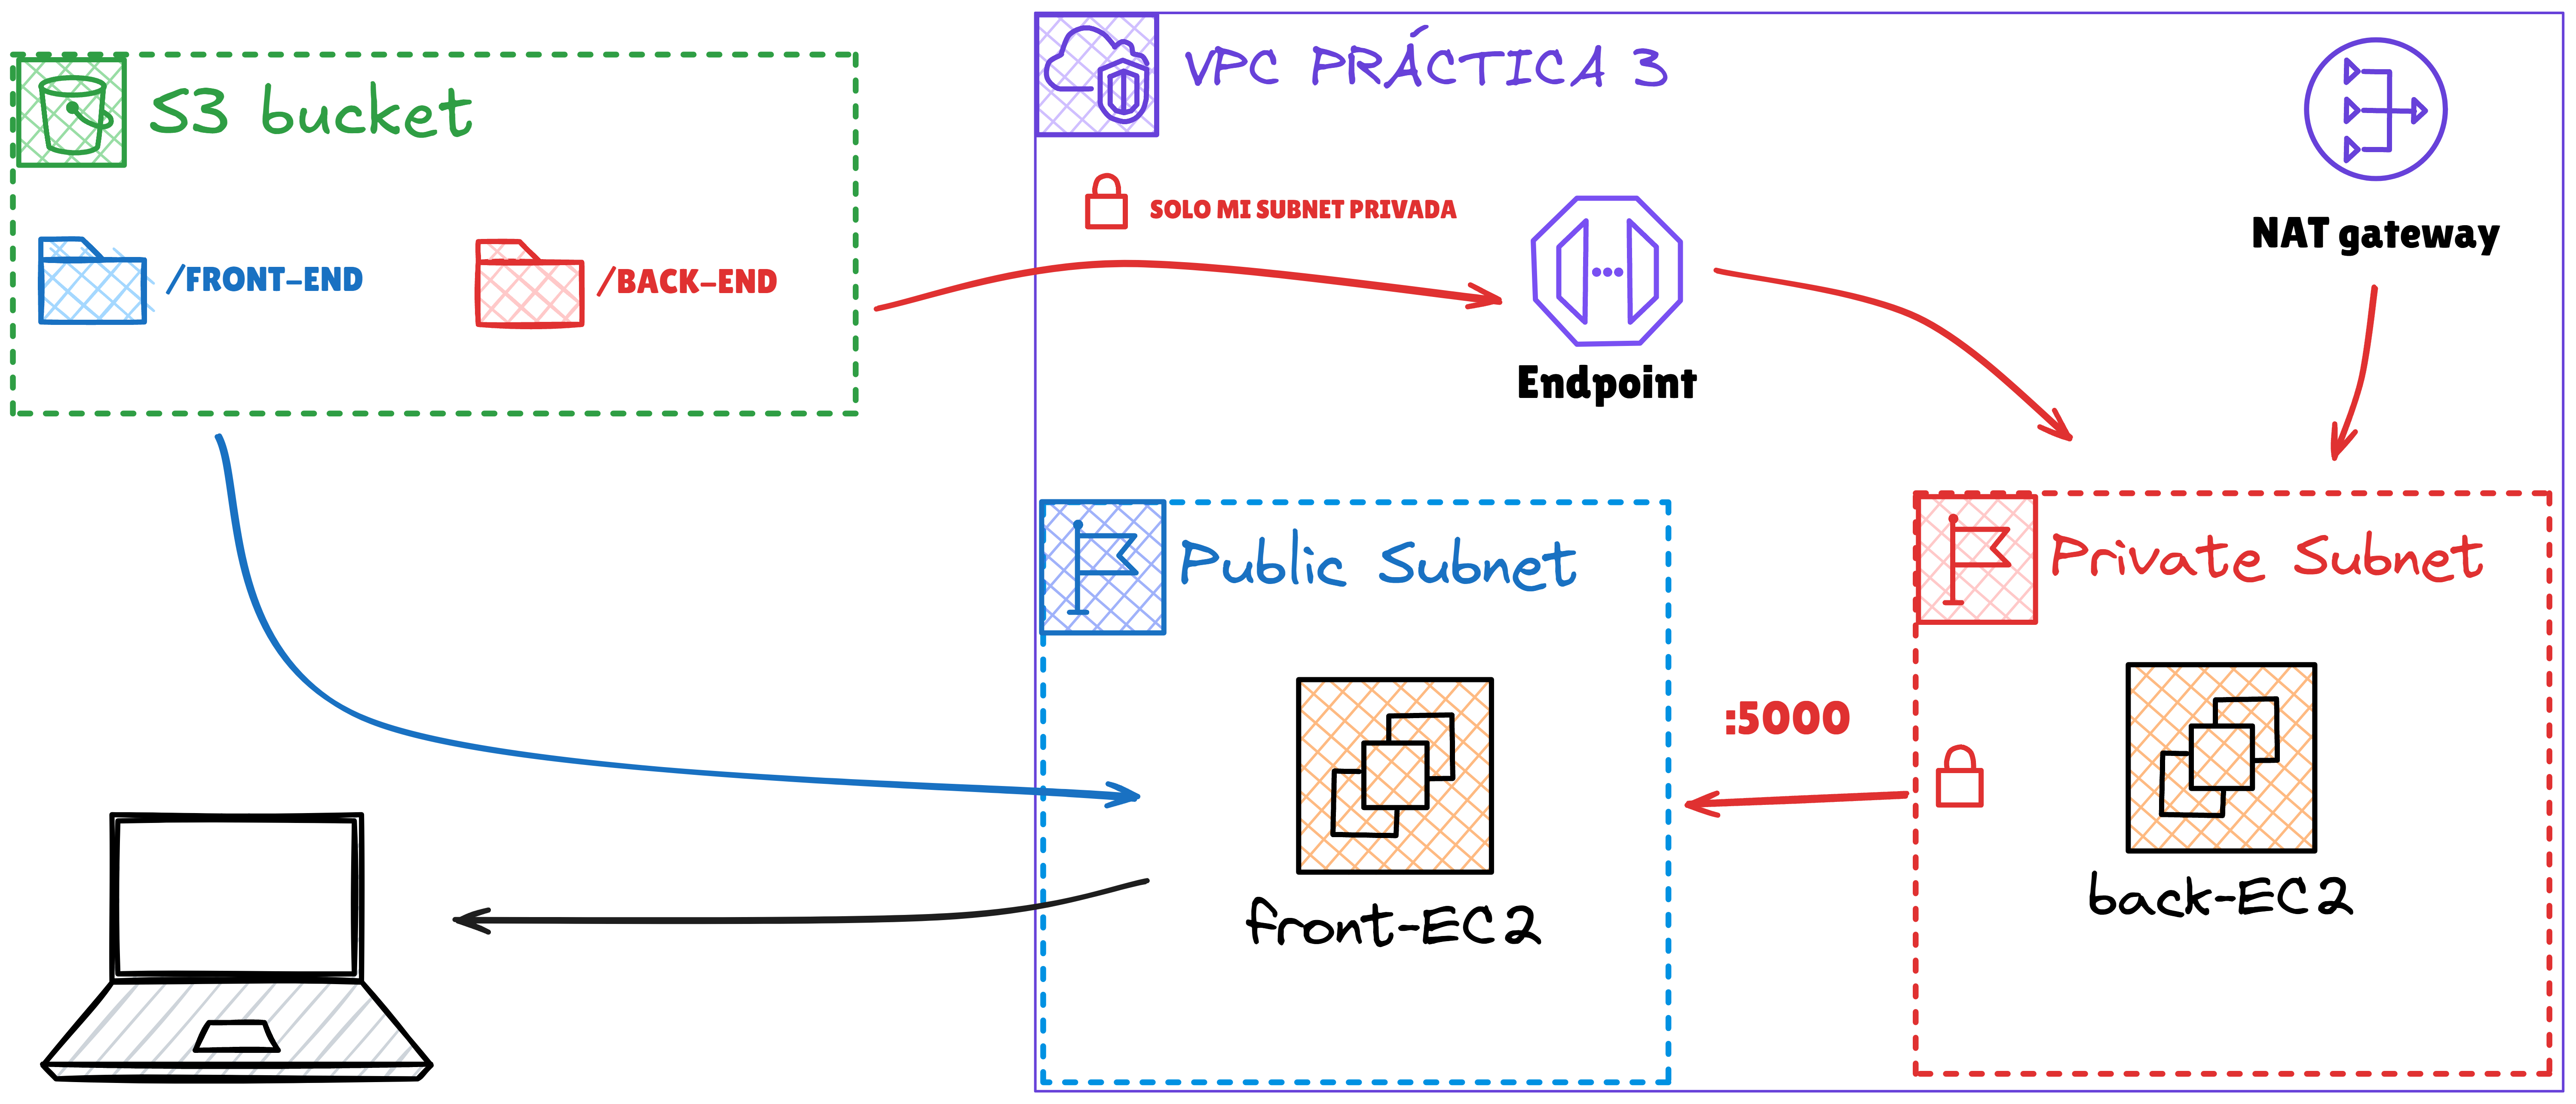
\includegraphics[width=1.1\textwidth]{esquema.png}}
	\end{figure}

	\newpage
	\tableofcontents

	\newpage

	\section{Configuración de la VPC}

	Una VPC es una red virtual aislada, cada cuenta de AWS contiene por defecto una VPC. Para poder controlar de una mejor forma las subredes que la conforman, los endpoints, las tablas de enrutamiento y los distintos servicios asociados que contienen, crearemos una nueva VPC y así tendremos acceso a la configuración de la VPC desde el principio.
		
	\subsection{Creación de las subredes}

	Para la práctica propuesta necesitaremos crear dos subredes, una pública donde tendremos nuestra instancia EC2 de frontend y el NAT Gateway. La instancia se utilizará para desplegar nuestra web y el Nat Gateway para conectar a internet las instancias de la subred privada. Finalmente la subred privada contará únicamente con la instancia del backend. Esta deberá de poder descargar librerías de internet y conectarse a la carpeta de backend del bucket S3 para desplegar la aplicación.
\\
\\
	Configuraremos la VPC con las dos subredes publicas y dos privadas de forma que tengamos dos zonas de disponibilidad para mejorar la estabilidad del sistema. Por ahora no configuraremos el Nat Gateway, lo crearemos posteriormente.

	\begin{figure}[H]
	\centering
	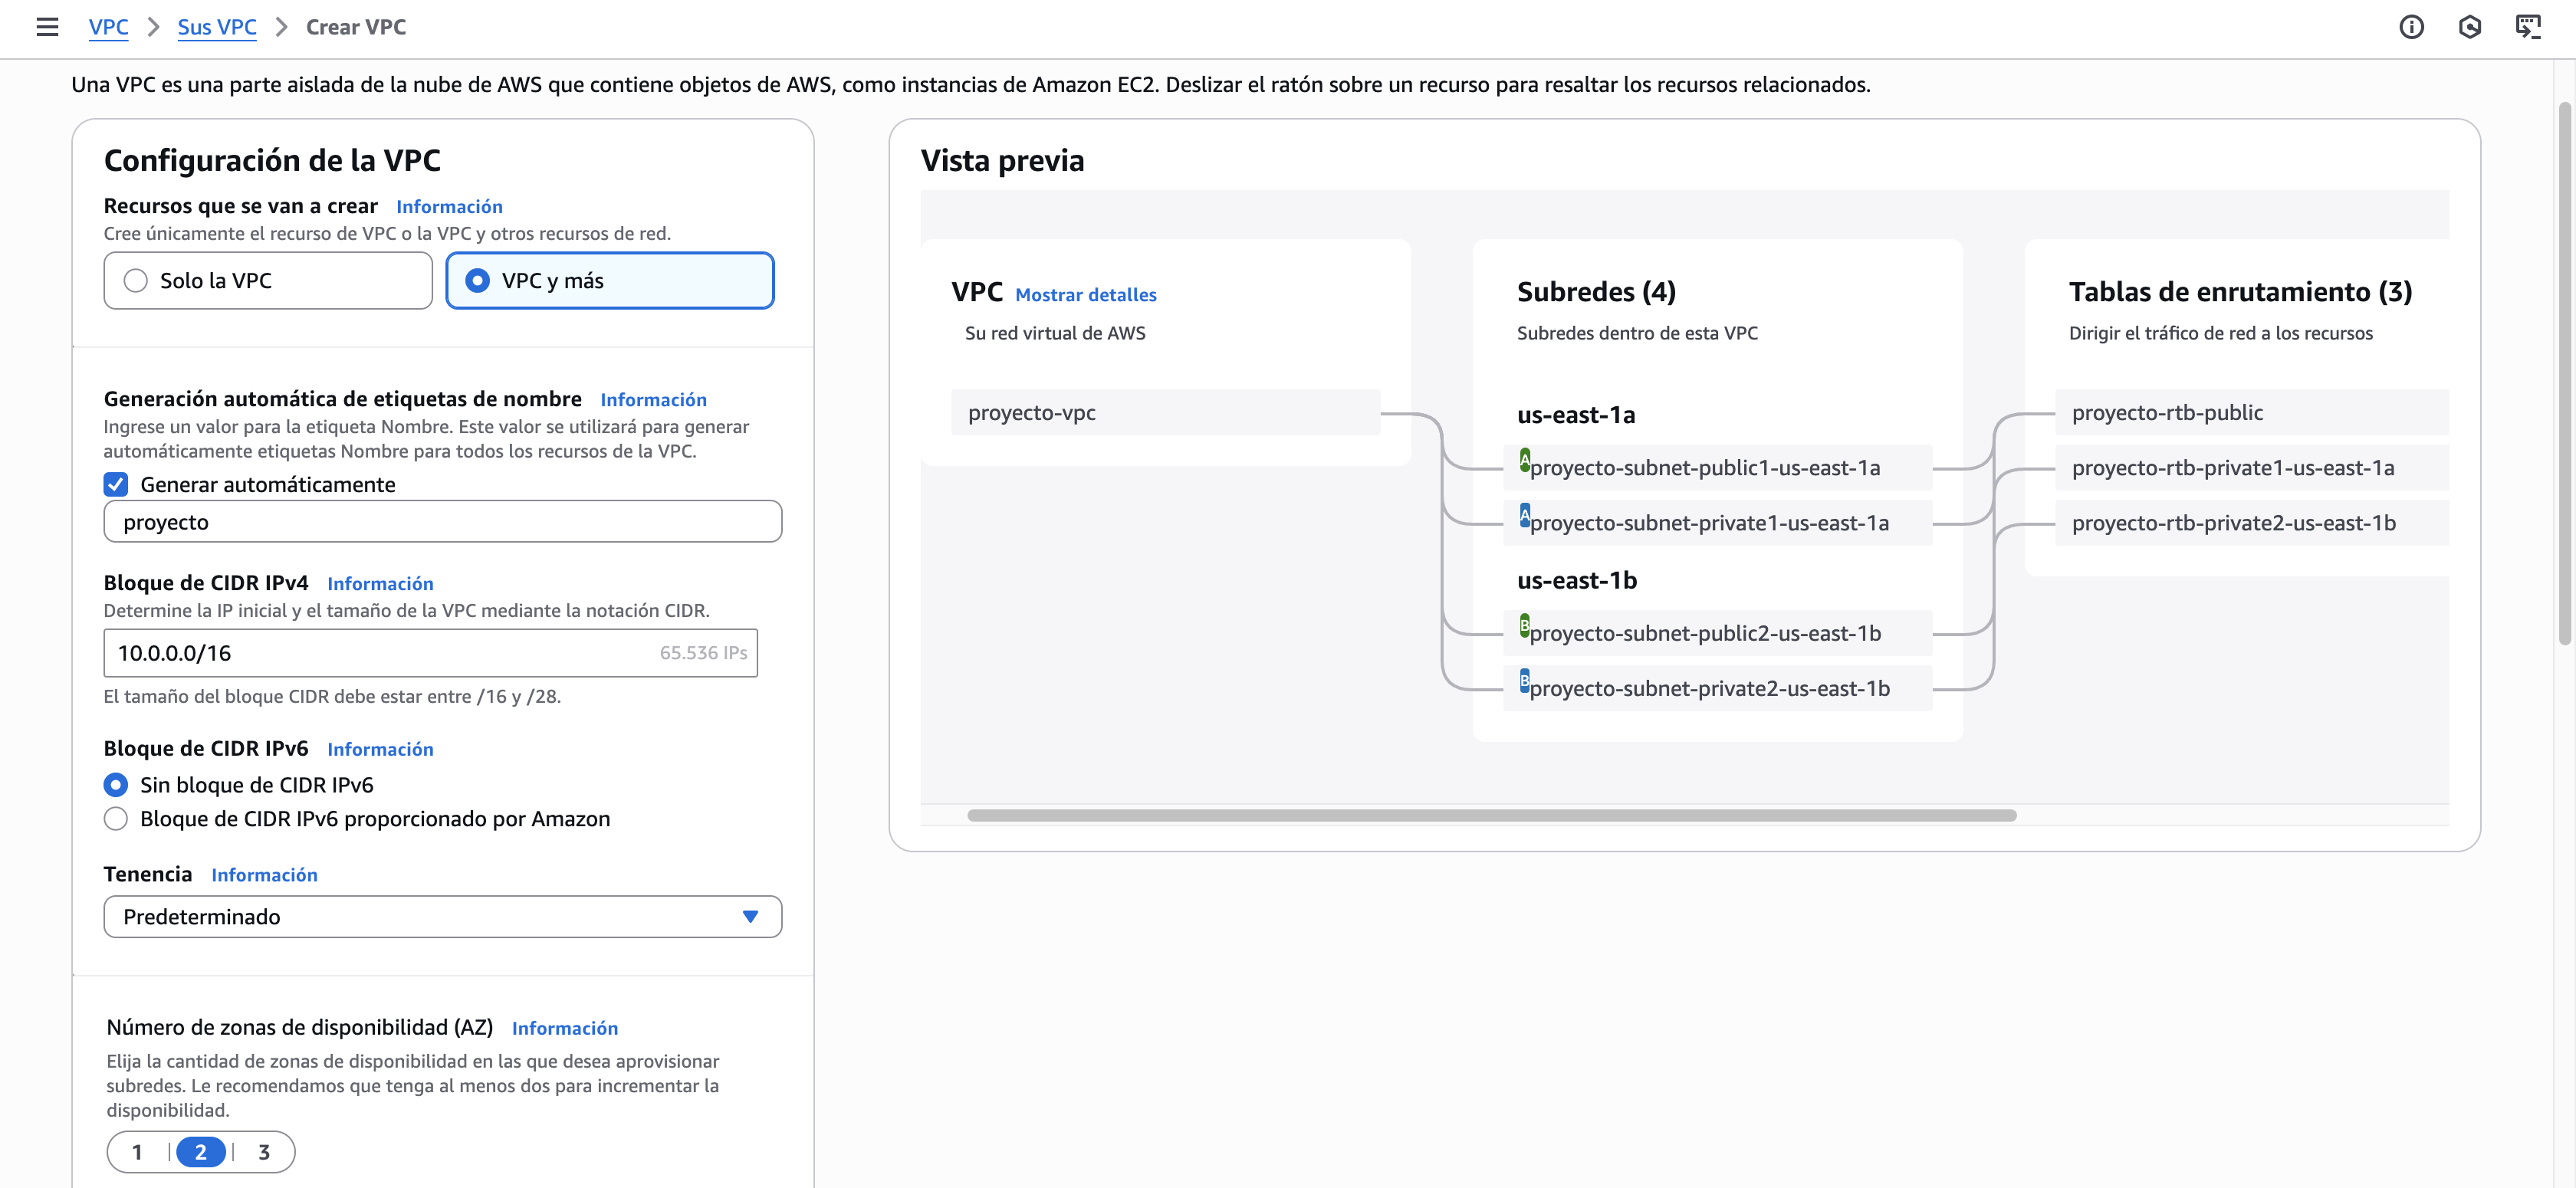
\includegraphics[width=0.95\textwidth]{configuracion_VPC.png}
	\caption{Configuración de la VPC}
	\end{figure}
	

	\subsection{Endpoint}

	Para que la instancia de la sub red privada descargue los archivos que tiene que ejecutar debe de poder conectarse a la parte privada del bucket (la carpeta /back-end), para ello lo primero que debemos de configurar será nuestra puerta de enlace (endpoint). El endpoint nos servirá como credencial para que las políticas del bucket nos proporcionen permisos al entrar desde este endpoint. El endpoint conectará las dos subredes privadas al completo con el servicio de AWS S3, de forma que permita la carga y descarga de recursos a cualquier bucket S3 dentro de la región de la VPC.
\\
\\
	En el apartado de crear punto de conexión elegiremos servicios AWS, seleccionaremos el servicio de S3 tipo Gateway, después escogemos nuestra VPC y por ultimo lo conectaremos a nuestras dos subredes privadas.

	\begin{figure}[H]
	\centering
	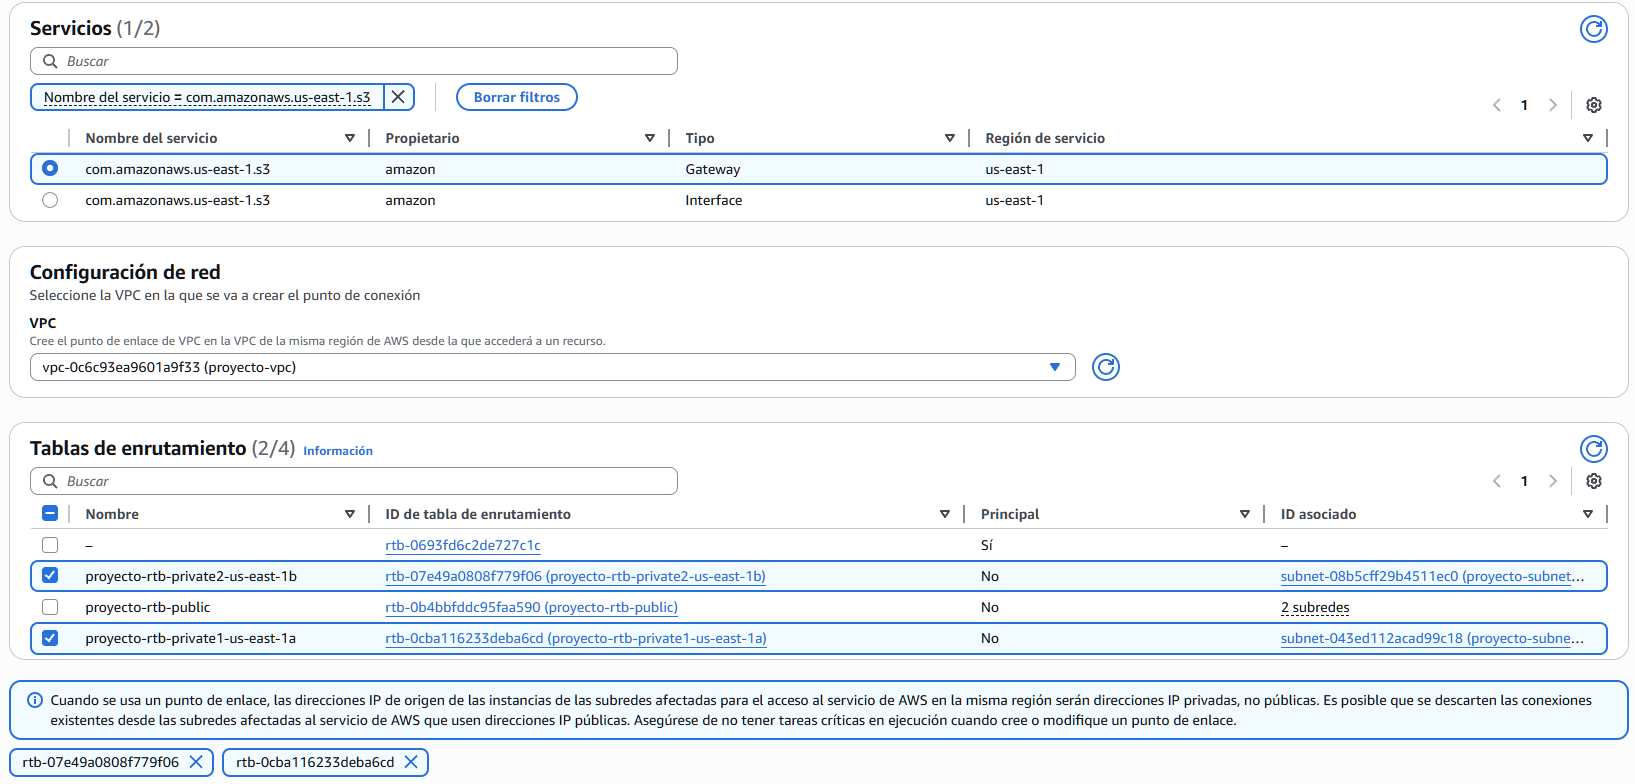
\includegraphics[width=0.95\textwidth]{crear_endpoint.png}
	\caption{Panel de crear endpoint}
	\end{figure}

	\subsection{NAT gateway}

	Para que una instancia en la subred privada pueda acceder a Internet (en nuestro caso, para descargar librerías), se debe usar un NAT Gateway. El NAT Gateway se despliega en una subred pública y utiliza el Internet Gateway (IGW) de la VPC. El IGW dirige el tráfico de Internet hacia el NAT Gateway, permitiendo la comunicación de carga y descarga saliente a Internet. Posteriormente veremos como conectarnos mediante las tablas de enrutamiento desde la subred privada.
	\\\\
	Podríamos no tener que configurar ningún NAT Gateway si las librerías que vayamos a usar las tuviéramos directamente en el bucket S3, de forma que solo nos haría falta el Endpoint S3 y nos saldría más barato el sistema en una práctica real.
\\\\
	Para crear el NAT Gateway debemos de clickar en el botón de crear gateway NAT y seleccionar la red publica de nuestra VPC. Para un entorno real debemos de crear un NAT Gateway por zona de disponibilidad, es decir, en nuestro caso dos.

	\begin{figure}[H]
	\centering
	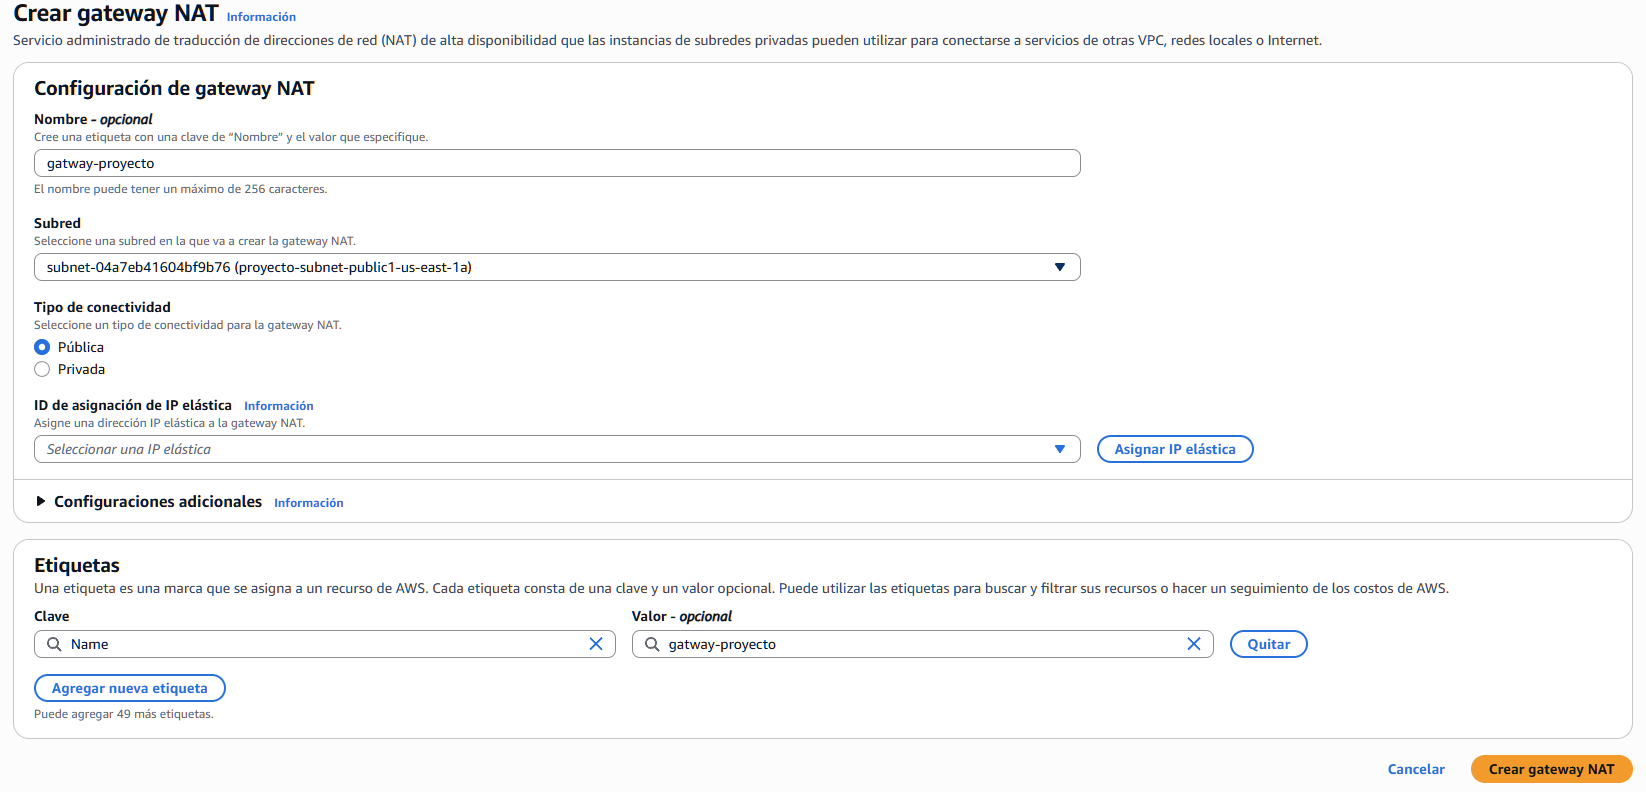
\includegraphics[width=0.95\textwidth]{crear_NAT_Gateway.png}
	\caption{Panel de crear gateway NAT}
	\end{figure}


	\subsection{Tablas de enrutamiento}

	Los dos servicios que hemos visto anteriormente (El Endpoint y el NAT Gateway) debemos de vincularlos para que la subred privada tenga acceso.
	\\\\ La forma de hacer esto es entrando dentro de las tablas de enrutamiento de las dos subredes privadas. El Endpoint S3 se vincula automáticamente al elegir las subredes en el momento de crearlo, y el NAT Gateway debemos de añadirlo editando las rutas de las tablas de enrutamiento y ingresando el nat-id que hemos creado.


	
	\begin{figure}[H]
	\centering
	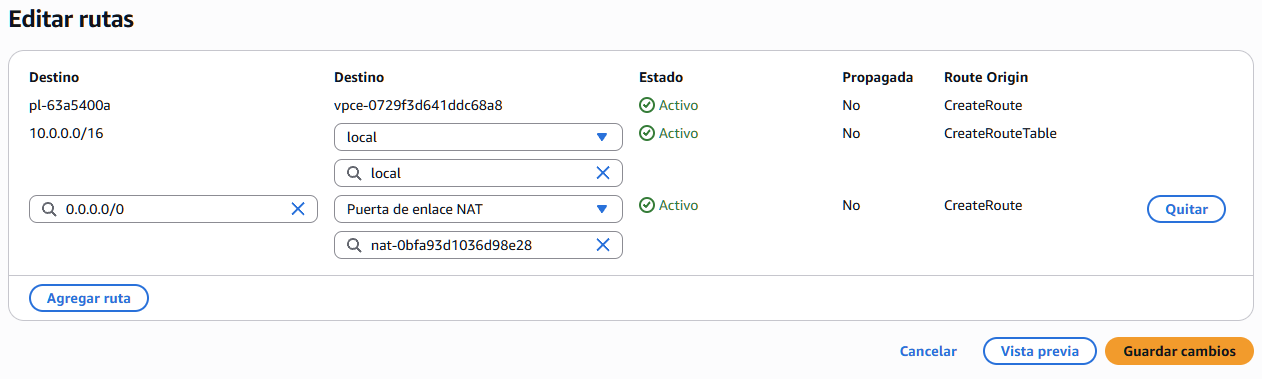
\includegraphics[width=0.95\textwidth]{editar_rutas.png}
	\caption{Panel de editar rutas}
	\end{figure}


	\section{Configuración del bucket S3}

	El bucket S3 debe de disponer de todo el código y archivos que necesiten las instancias para poder ser ejecutadas y funcionar correctamente. Al mismo tiempo debemos asegurarnos de restringir el acceso para evitar accesos no autorizados y minimizar el riesgo de ataque informático. Crearemos un bucket con un nombre único (el mio se llamará \fbox{backeet-p3}) y usaremos el almacenamiento de uso general. Posteriormente configuraremos la seguridad del almacenamiento.

	
	\begin{figure}[H]
	\centering
	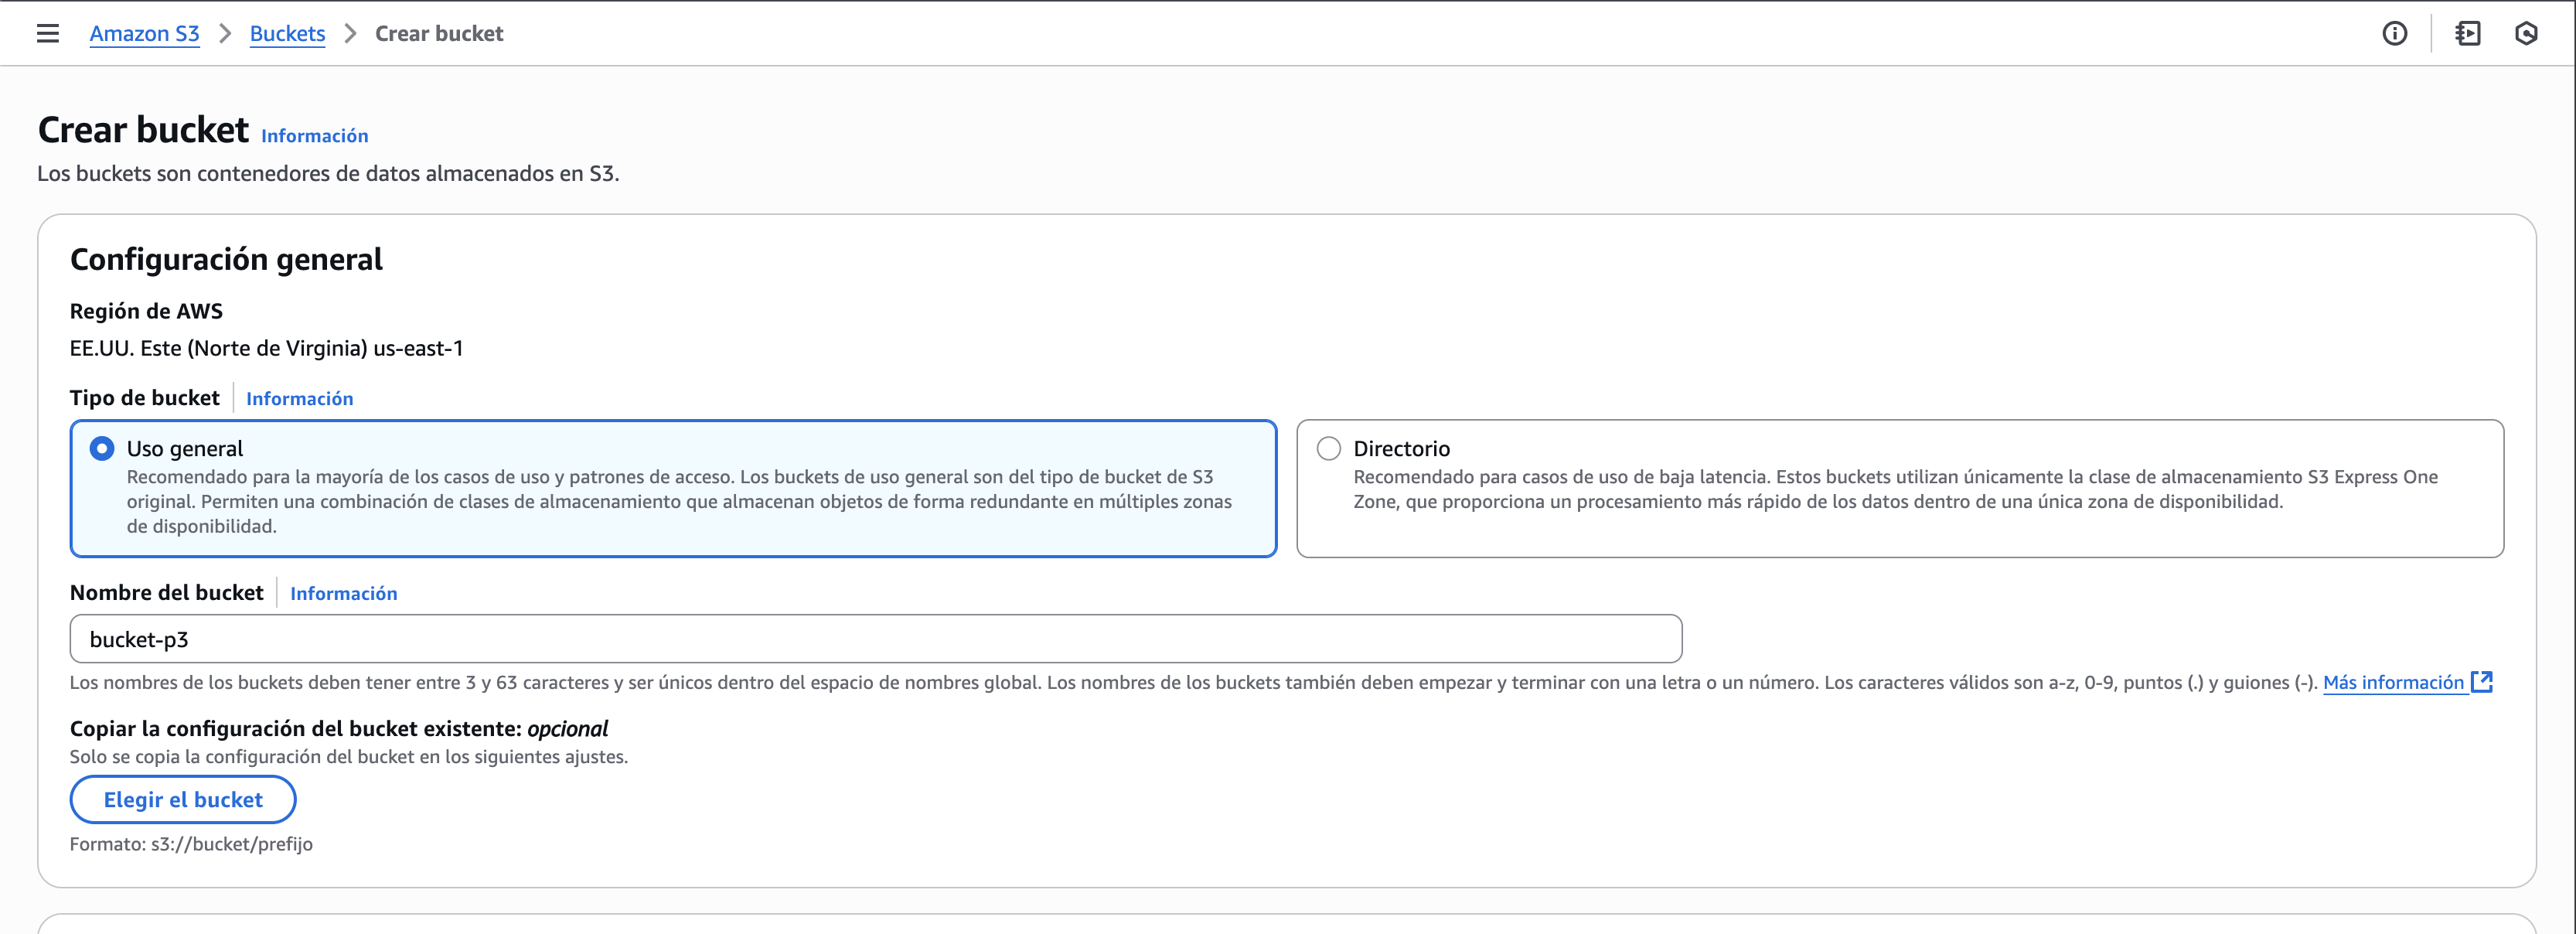
\includegraphics[width=0.95\textwidth]{crear_bucket.png}
	\caption{Panel de crear bucket}
	\end{figure}

	\subsection{/Front-end}

	Los archivos de ``\verb|index.html|'' y ``\verb|app_front.js|''  los guardaremos en una carpeta pública, la carpeta \fbox{front-end}, esta carpeta será accesible desde cualquier lugar. De esta forma no hace falta utilizar ningún endpoint que sirva como credencial, ni ningún rol para descargar estos archivos en nuestra instancia.
	\\\\
	Primero le daremos a crear carpeta y posteriormente le asignaremos un nombre y cargaremos los archivos mencionados anteriormente.

	
	\begin{figure}[H]
	\centering
	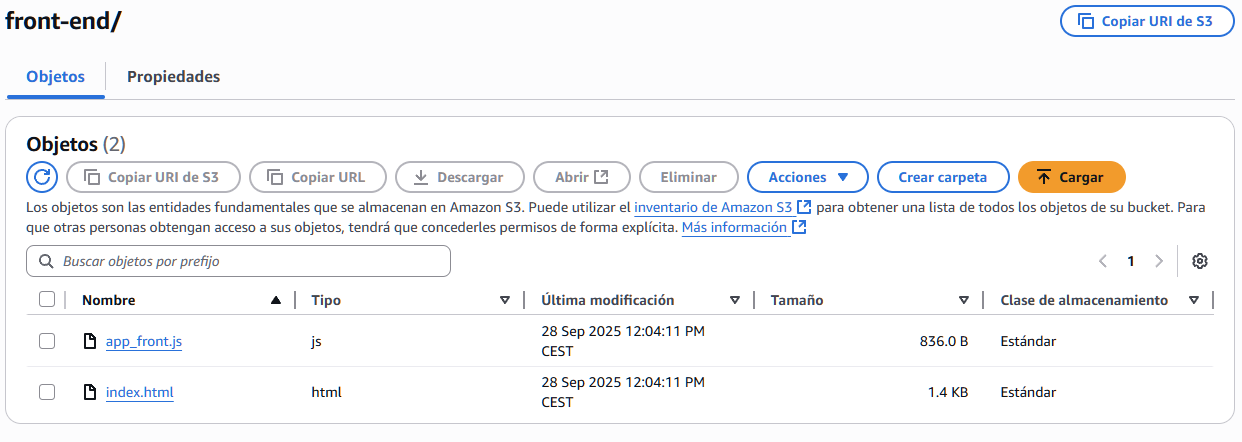
\includegraphics[width=0.95\textwidth]{archivos_s3_front.png}
	\caption{Archivos S3 /front-end}
	\end{figure}

	\subsection{/Back-end}

	Para la parte de la lógica de negocio y datos sensibles (como nuestro modelo de inferencia), crearemos otra carpeta, esta privada, la carpeta \fbox{back-end}. En nuestro caso los archivos ``\verb|app_backend.py|'' y el ``\verb|modelo.pkl|'' son los más críticos, por lo que debemos de controlar estrictamente el acceso a esta carpeta. 
	\\\\
	Haremos lo mismo que con la carpeta anterior, la crearemos y subiremos nuestros archivos. La seguridad de esta carpeta la manejaremos en el paso siguiente.


	
	\begin{figure}[H]
	\centering
	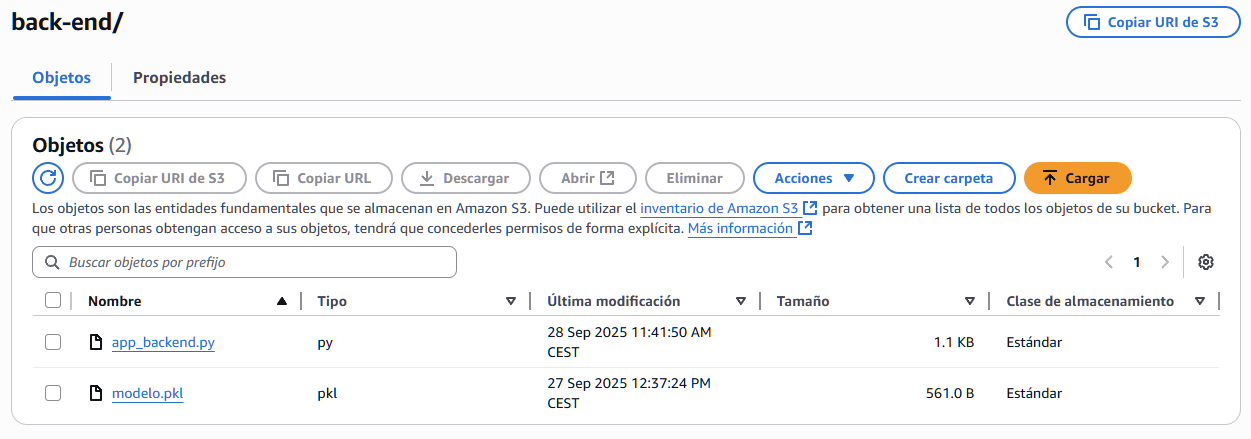
\includegraphics[width=0.95\textwidth]{archivos_s3_bck.png}
	\caption{Archivos S3 /back-end}
	\end{figure}

	\subsection{Permisos y políticas}

	Esta es la parte más importante en la creación del bucket. Anteriormente al crear el bucket, por defecto hemos bloqueado el acceso público al S3. Lo que debemos de hacer ahora es abrir los accesos, y mediante la política del bucket permitir únicamente el acceso a descargar los archivos de la carpeta /back-end que provengan del Endpoint que hemos creado anteriormente. Esto lo que hará será permitir los accesos a la carpeta de todas las instancias que se encuentren dentro de nuestra red privada. 
	\\\\
	Al crear una política restringida, la carpeta de /front-end no será accesible, ya que se aplica el principio de denegación por defecto, esto significa que si una acción no está explícitamente permitida, estará denegada. Por lo que permitiremos el acceso a descargar los archivos de la carpeta /front-end a todos los usuarios también en la política del bucket.
	\\\\
	Nos dirigiremos dentro de nuestro bucket a permisos, desbloquearemos el permiso de accesos públicos y editaremos la política para que la acción GetObject se permita utilizar dentro de baqueet-p3/back-end/ solamente desde nuestra vpce anterior añadiendo la condición de StringEquals. Posteriormente hacemos lo mismo con la carpeta del front-end pero sin usar ninguna condición. De este modo queda la carpeta back-end restringida y accesible únicamente mediante el subnet privado y la carpeta front-end abierta a todo el mundo.
	\\\\
<<<<<<< HEAD
	Otra forma de hacerlo sin usar roles sería usando la ip privada de la instancia y hacer que se permita el acceso solamente si coincide la ip de la política con la ip de la instancia. Esto no es muy util en nuestro caso ya que estaríamos cambiando la política todo el rato y no podríamos usar de manera correcta los UserData de las instancias, al ejecutar primero la instancia sin saber la IP privada no habría tiempo físico para cambiarla en el bucket. 
=======
	Otra forma de hacerlo sin usar roles sería usando la ip privada de la instancia y hacer que se permita el acceso solamente si coincide la ip de la política con la ip de la instancia. Esto no es muy util en nuestro caso ya que estaríamos cambiando la política todo el rato y no podríamos usar de manera correcta los UserData de las instancias.
>>>>>>> 42fa237a0948d1ceb29232ede3f74fd9ab574339


	

	\begin{lstlisting}[style=consola, language=bash, caption={política-s3.json}]
{
    "Version": "2012-10-17",
    "Statement": 
    [
        {
            "Sid": "AllowBackendFromVPCEndpoint",
            "Effect": "Allow",
            "Principal": "*",
            "Action": "s3:GetObject",
            "Resource": "arn:aws:s3:::baqueet-p3/back-end/*",
            "Condition": 
            {
                "StringEquals": 
				{"aws:SourceVpce": "vpce-05b2e68f0d4435792"}
            }
        },
        {
            "Sid": "PublicReadForFrontEndAssets",
            "Effect": "Allow",
            "Principal": "*",
            "Action": "s3:GetObject",
            "Resource": "arn:aws:s3:::baqueet-p3/front-end/*"
        }
    ]
}\end{lstlisting}

	\section{Instancias}
<<<<<<< HEAD
	Las instancias serán desplegadas dentro de nuestra VPC, la instancia que ejecute el front será desplegada en la subnet pública mientras que la instancia que ejecute el back será ejecutada en la subnet privada. Para que sea menos tedioso el despliegue utilizaremos los User Data, es un archivo .sh que se ejecutan al crear cada instancia. Estos User Data tendrán sentencias ``echo'' para que cuando nos metamos a monitorear y comprobar los logs de cada instancia sepamos en que ha fallado de manera rápida y práctica.
=======
	Las instancias serán desplegadas dentro de nuestra VPC, la instancia que ejecute el front será desplegada en la subnet pública mientras que la instancia que ejecute el back será ejecutada en la subnet privada. Para que sea menos tedioso el despliegue utilizaremos los User Data, es un archivo .sh que se ejecutan al iniciar cada instancia. Estos User Data tendrán sentencias ``echo'' para que cuando nos metamos a monitorear y comprobar los logs de cada instancia sepamos en que ha fallado de manera rápida y práctica.
>>>>>>> 42fa237a0948d1ceb29232ede3f74fd9ab574339

	\subsection{Grupos de Seguridad}
	Lo primero que tenemos que hacer antes de lanzar las instancias será crear dos grupos de seguridad, uno para el frontend el que permita  todas las entradas http y otro para el backend que unicamente permita entradas del grupo de seguridad del frontend mediante un TCP personalizado en el puerto 5000 que es el que usaremos para lanzar el back.

		
	\begin{figure}[H]
	\centering
	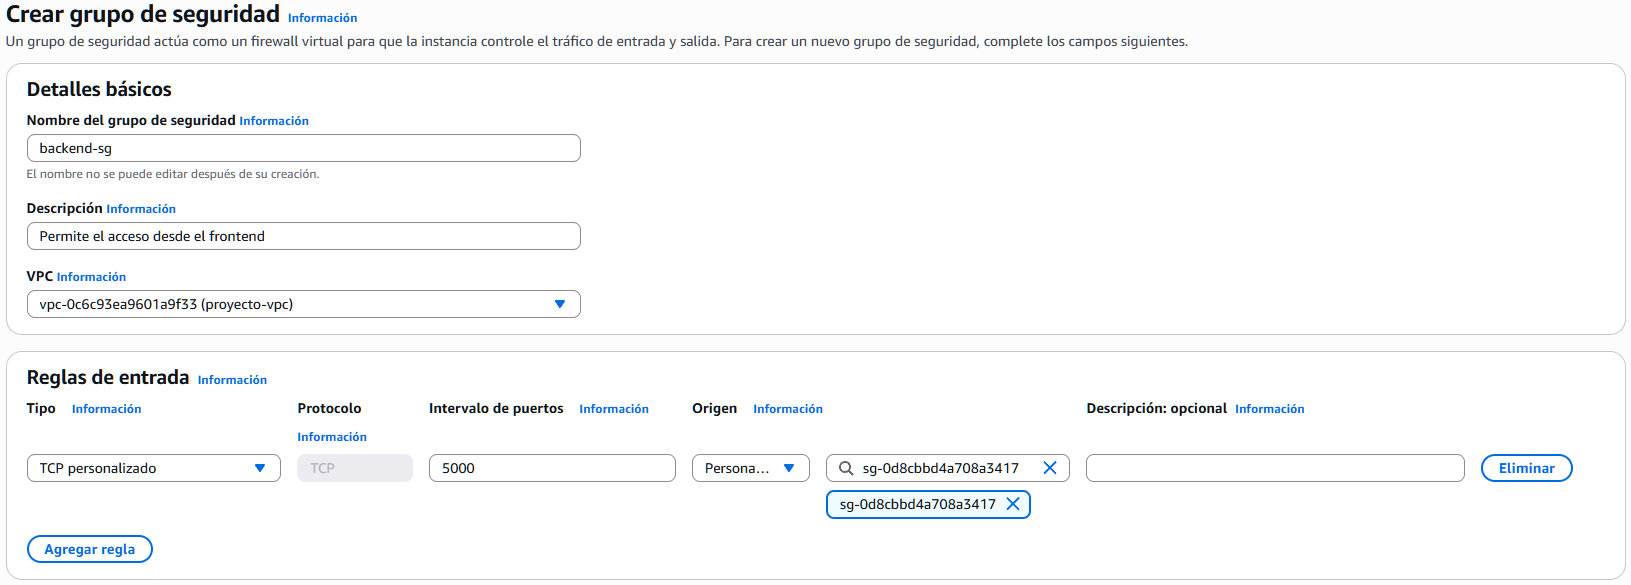
\includegraphics[width=0.95\textwidth]{reglas_gr_privado.png}
	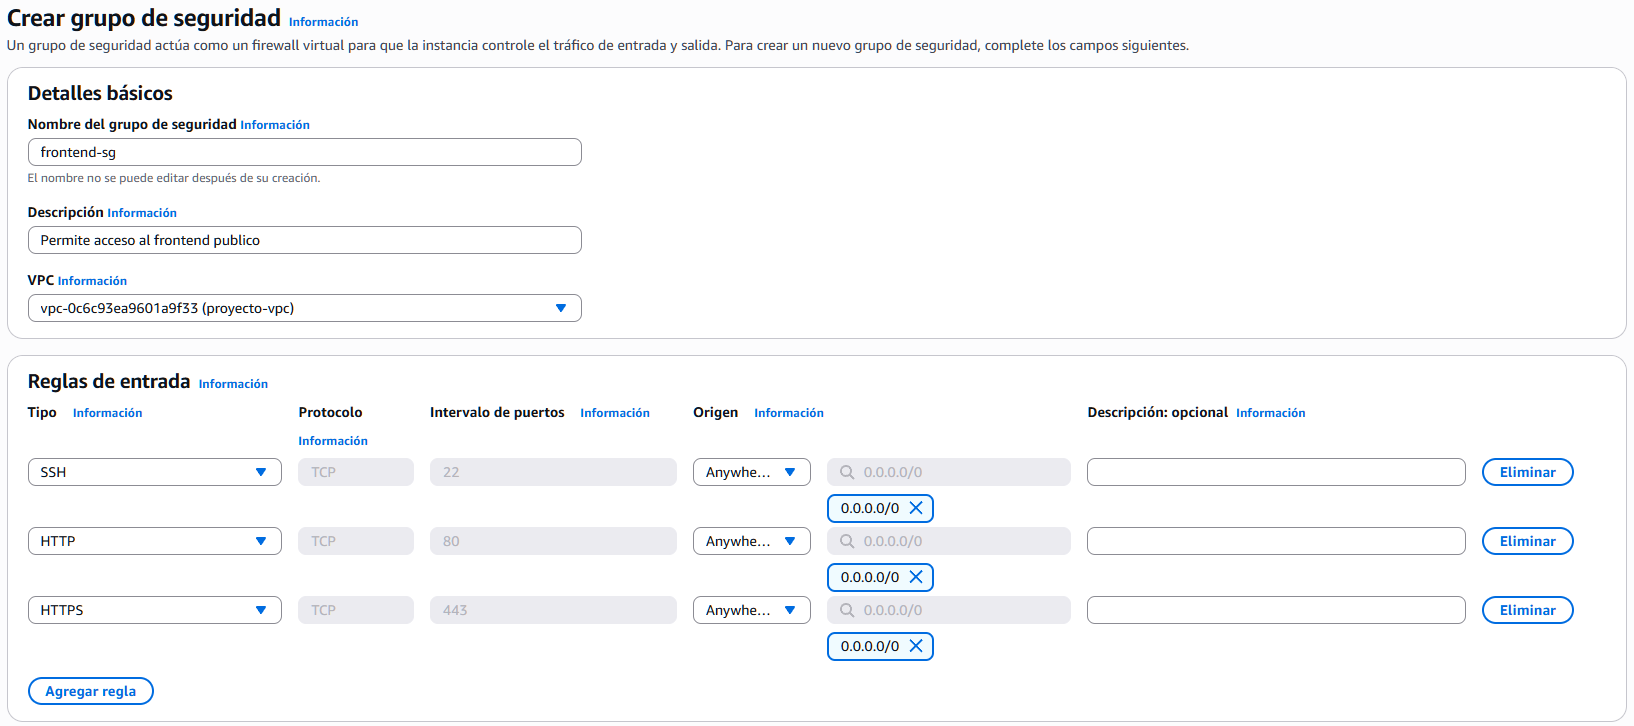
\includegraphics[width=0.95\textwidth]{reglas_gr_publico.png}
	\caption{Reglas de los grupos privado y público}
	\end{figure}

	\subsection{Instancia backend}
	La instancia backend contará con un par de lleves, elegiremos nuestra VPC y nuestra subred privada, posteriormente le asignaremos el grupo de seguridad de la sección anterior y deshabilitaremos la asignación de ip publica ya que nuestra instancia backend solo va a ser accesible mediante su ip privada desde el puerto 5000 y desde el frontend. Es por esto también por lo que creamos primero el backend, asi sabremos nuestra dirección ip privada cuando se despliegue el back y podremos cambiar el archivo del front javascript a la ip correspondiente.

			
	\begin{figure}[H]
	\centering
	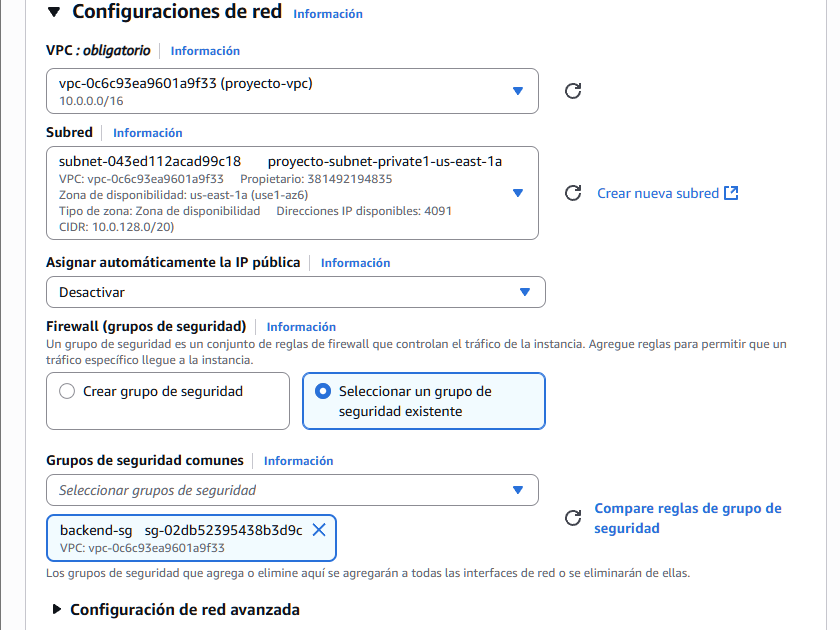
\includegraphics[width=0.82\textwidth]{configuracion_ec2_back.png}
	\caption{Configuración ec2 back}
	\end{figure}

	\subsubsection{Back User Data}
	El siguiente .sh el user data que voy a utilizar, se configura en la parte final de detalles avanzados al crear la instancia. En él instalaremos todas las dependencias que necesite nuestra aplicación back, crearemos los directorios para alojar los archivos, descargaremos los archivos del S3 y desplegaremos el servidor ejecutando el archivo python. Todo esto se hará automáticamente cuando se inicie la instancia. 

	\begin{lstlisting}[style=python-style, caption= back user data sh]
	#!/bin/bash

	echo "--- Iniciando script de User Data para el Back-End ---"

	# 1. Actualizar sistema e instalar Python y pip
	echo "Actualizando sistema e instalando Python y pip..."
	yum update -y
	yum install python3-pip -y
	echo "Python y pip instalados."

	# 2. Instalar dependencias de Python necesarias para la aplicación
	echo "Instalando dependencias de Python (Flask, joblib, scikit-learn)..."
	pip3 install flask joblib scikit-learn
	echo "Dependencias de Python instaladas."

	# 3. Crear directorios para la aplicación
	echo "Creando directorios de la aplicación en /app..."
	mkdir -p /app
	cd /app
	echo "Directorio creado y nos hemos movido a /app."

	# 4. Descargar los archivos del back-end desde S3 usando wget
	echo "Descargando archivos del back-end desde S3..."
	wget -O app_backend.py https://baqueet-p3.s3.us-east-1.amazonaws.com/back-end/app_backend.py
	wget -O modelo.pkl https://baqueet-p3.s3.us-east-1.amazonaws.com/back-end/modelo.pkl

	# 5. Verificar que los archivos existen antes de continuar
	if [ ! -f "app_backend.py" ] || [ ! -f "modelo.pkl" ]; then
		echo "ERROR: Uno o ambos archivos del back-end no se encontraron después de la descarga."
		exit 1
	fi

	# 6. Ejecutar el servidor de Flask en segundo plano
	echo "Iniciando el servidor de Flask..."
	python3 app_backend.py &

	echo "--- Script de User Data del Back-End finalizado con éxito. ---"

	\end{lstlisting}

	\subsubsection{Back Logs}
<<<<<<< HEAD
	Cuando nos salgan los siguientes logs dentro del monitoreo de la instancia sabremos que tenemos el servidor desplegado sin errores por el momento.
=======
	Cuando nos salgan los siguientes logs dentro del monitoreo de la instancia sabremos que tenemos el servidor desplegado sin errores.
>>>>>>> 42fa237a0948d1ceb29232ede3f74fd9ab574339

	\begin{lstlisting}[style=consola, language=bash, caption={back logs}]
	[   44.966280] cloud-init[1633]:  * Serving Flask app 'app_backend'
	[   44.966623] cloud-init[1633]:  * Debug mode: off
	[   44.978437] cloud-init[1633]: WARNING: This is a development server. Do not use it in a production deployment. Use a production WSGI server instead.
	[   44.978585] cloud-init[1633]:  * Running on all addresses (0.0.0.0)
	[   44.978809] cloud-init[1633]:  * Running on http://127.0.0.1:5000
	[   44.979093] cloud-init[1633]:  * Running on http://10.0.142.191:5000
	[   44.979476] cloud-init[1633]: Press CTRL+C to quit\end{lstlisting}

	\subsection{Instancia frontend}

	Por el otro lado la instancia del frontend contará con el mismo par de llaves y la misma VPC, elegiremos una de las subredes públicas y habilitaremos la opción de asignar IP pública, elegiremos el grupo de seguridad del frontend y cargaremos nuestro User Data. 

		
	\begin{figure}[H]
	\centering
	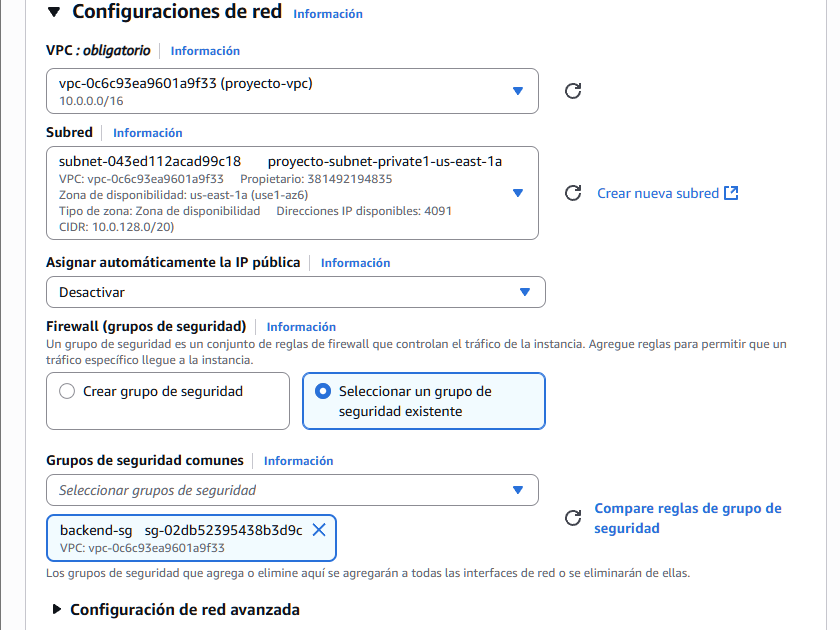
\includegraphics[width=0.95\textwidth]{configuracion_ec2_back.png}
	\caption{Configuración EC2 back}
	\end{figure}

	
	
	\newpage
	\subsubsection{Front User Data}

	Para este otro user data debemos de hacer una modificación y pegar la ip privada del backend en la sentencia sed que remplaza la string de \verb|IP_PRIVADA_DEL_BACKEND| (que se encuentra dentro del código javascript) por nuestra ip privada. Haciéndolo de este modo nos olvidamos de estar modificando el archivo dentro del bucket S3. El sh hará lo mismo que el anterior, descargar dependencias he instalarlas, descargar el código del S3 y ejecutarlo. Como vemos en los User Data usamos siempre ``wget'' en vez de ``aws s3'', esto lo hacemos porque solamente hemos permitido la acción de GetObject en la política del S3.
	
	\begin{lstlisting}[style=python-style, caption= front user data sh]
	#!/bin/bash

	echo "--- Iniciando script de User Data para el Front-End ---"

	# 1. Actualizar sistema e instalar Node.js desde el repositorio de NodeSource
	echo "Actualizando sistema e instalando Node.js..."
	yum update -y
	# Añadir el repositorio de Node.js 18
	curl -fsSL https://rpm.nodesource.com/setup_18.x | bash -
	# Instalar Node.js (incluye npm)
	yum install -y nodejs
	# Instalar dependencias globales
	npm install -g express axios
	echo "Node.js instalado."

	# 2. Crear directorios, descargar archivos e instalar dependencias
	echo "Creando directorios de la aplicación en /app..."
	mkdir -p /app/public
	cd /app
	echo "Directorio creado y nos hemos movido a /app."

	# 3. Descargar los archivos del front-end desde S3
	# ... (tus comandos wget van aquí) ...
	wget -O app_front.js https://baqueet-p3.s3.amazonaws.com/front-end/app_front.js
	wget -O ./public/index.html https://baqueet-p3.s3.amazonaws.com/front-end/index.html
	echo "Archivos descargados."

	# Instalar dependencias LOCALMENTE
	echo "Instalando dependencias de Node.js..."
	npm install express axios
	echo "Dependencias instaladas."

	# 4. Verificar que los archivos existen antes de continuar
	if [ ! -f "app_front.js" ] || [ ! -f "./public/index.html" ]; then
		echo "ERROR: Uno o ambos archivos del front-end no se encontraron después de la descarga."
		exit 1
	fi

	# 5. Reemplazar la IP del backend en el archivo de la aplicación
	echo "Reemplazando la IP del backend"
	sed -i 's/IP_PRIVADA_DEL_BACKEND/10.0.142.191/g' app_front.js
	echo "IP reemplazada."

	# 6. Ejecutar el servidor de Node.js en segundo plano
	echo "Iniciando el servidor de Node.js..."

	node app_front.js &

	echo "--- Script de User Data del Front-End finalizado con éxito. ---"\end{lstlisting}
	\subsubsection{Front Logs}
<<<<<<< HEAD
	Cuando nos salga el siguiente log sabremos que tendremos el servidor desplegado.
=======
	Cuando nos salgan los siguientes logs dentro del monitoreo de la instancia sabremos que tenemos el servidor desplegado sin errores.
>>>>>>> 42fa237a0948d1ceb29232ede3f74fd9ab574339

 	\begin{lstlisting}[style=consola, language=bash, caption={front logs}]
	[   39.309930] cloud-init[1633]: Cloud-init v. 22.2.2 finished at Wed, 01 Oct 2025 21:42:02 +0000. Datasource DataSourceEc2.  Up 39.29 seconds
	[   39.687491] cloud-init[1633]: Servidor front-end escuchando en el puerto 80 \end{lstlisting}

	\section{Mejora de la aplicación}

	Para mejorar la aplicación se me ocurrió la idea de lanzar otro tipo de servicio cambiando unicamente la parte de código de front y el modelo. Quería lanzar un modelo barato de ejecutar y a la vez más util que la regresión lineal, asi que se me ocurrió usar un modelo de análisis de sentimientos que te dijera si una frase de un comentario de cualquier tipo era buena o mala. Para hacer esto simplemente vamos a dejar la estructura del proyecto tal como está y unicamente cambiaremos los archivos del S3.

	\subsection{Frontend}
	Para el frontend usaremos un html más bonito con ayuda de la IA y el javascript le cambiamos unicamente el mensaje de error.

			
	\begin{figure}[H]
	\centering
	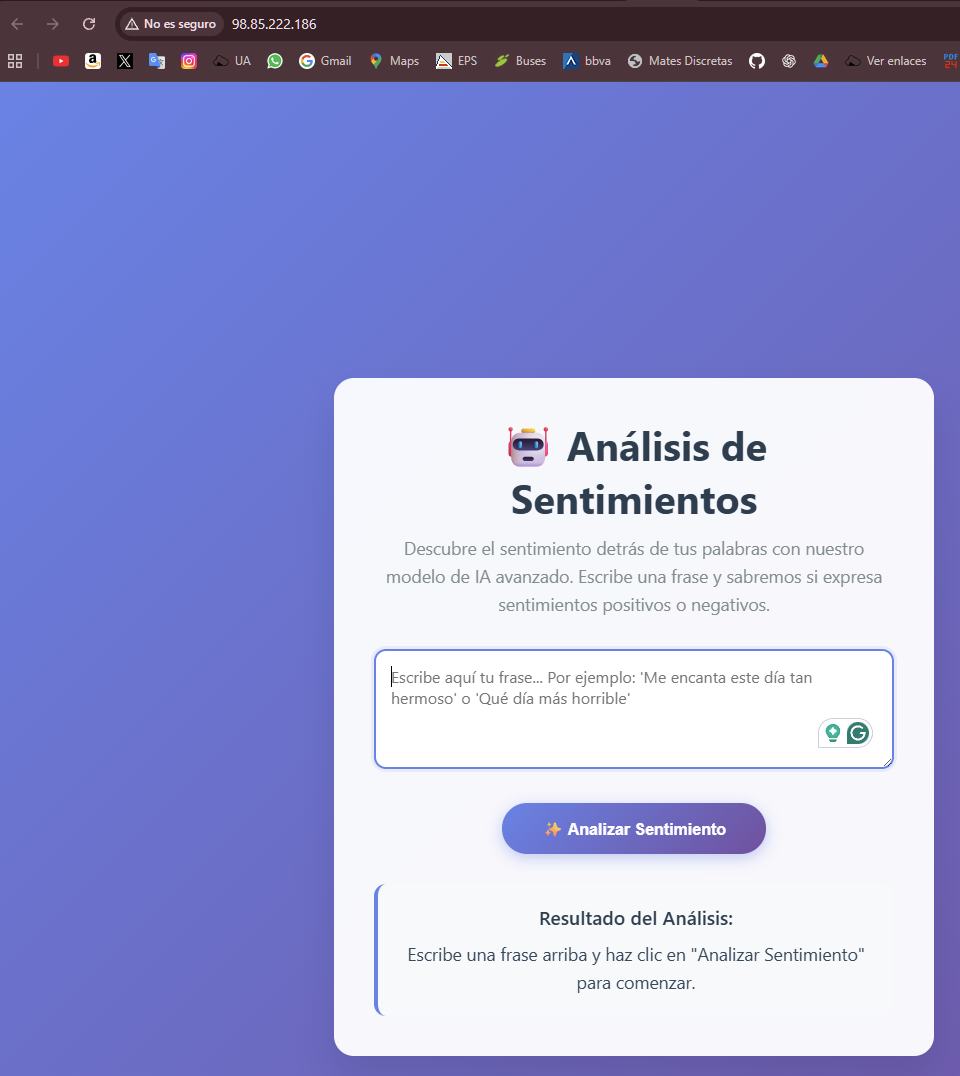
\includegraphics[width=0.55\textwidth]{prueba1.png}
	\caption{index html}
	\end{figure}

	\subsection{Backend}

	Para el backend busqué en internet el siguiente modelo de análisis de comentarios \href{https://github.com/sentiment-analysis-spanish/sentiment-spanish}{sentiment-spanish}, es muy ligero de 28 mb en total, contiende dos modelos uno para vectorizar las frases y el otro para clasificar este conjunto de vectores en positivos o negativos. Para poder ejecutarlo correctamente modificaré \verb|app_backend.py| y incluiré el código de dentro del repositorio que se usa para la predicción. También debemos de incluir en el user data del back las librerías nuevas que se van a usar, en nuestro caso: \verb|python3-devel, gcc, scikit-learn==0.23.2, numpy y pandas|. La carpeta /back-end quedaría con esta estructura final.

	\begin{lstlisting}[style=consola, language=bash, caption={/back-end}]
 /app/
  ├─ app_backend.py
  └─ saved_model/
    ├─ classifier_naive_bayes_compressed.pbz2
    └─ ngram_vectorized_compressed.pbz2\end{lstlisting}


	\section{Pruebas}

	En esta sección comprobaremos que las instancias funcionen y que los accesos al bucket estén controlados y restringidos.

	\subsection{Accesos al bucket}

<<<<<<< HEAD
	Para poder comprobar rápidamente si tenemos acceso a los archivos del bucket podemos ir a nuestro S3 y copiar los links de cada archivo que tengamos y pegarlos en el navegador. Como es lógico los archivos que tendremos dentro de nuestra carpeta /back-end, al no conectarnos mediante el endpoint y estar fuera de la subred privada, serán inaccesibles mientras que los que tengamos dentro de la carpeta /frontend podremos visualizarlos.
=======
	Para poder comprobar rápidamente si tenemos acceso a los archivos del bucket podemos ir a nuestro S3 y copiar los links de cada archivo que tengamos y pegarlos en el navegador. Como es lógico los archivos que tendremos dentro de nuestra carpeta /back-end al no conectarnos mediante el endpoint y estar fuera de la subred privada serán inaccesibles mientras que los que tengamos dentro de la carpeta /frontend podremos visualizarlos.
>>>>>>> 42fa237a0948d1ceb29232ede3f74fd9ab574339

	\begin{figure}[H]
	\centering
	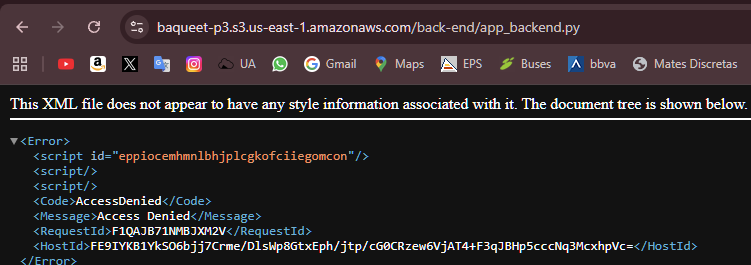
\includegraphics[width=0.95\textwidth]{acceso_denegado_back.png}
	\caption{acceso denegado back}
	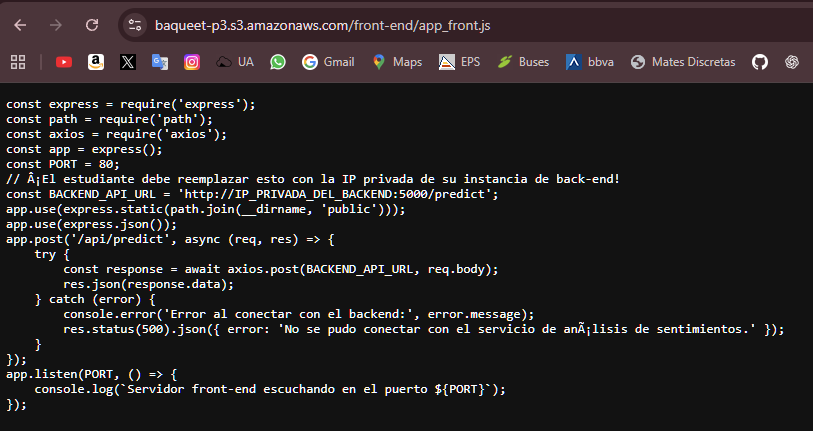
\includegraphics[width=0.95\textwidth]{acceso_publico_front.png}
	\caption{acceso público front}
	\end{figure}

	\newpage

	\subsection{Prueba de despliegue 1}
	Para poder conectarnos a nuestro frontend debemos de buscar la ip pública de nuestra instancia, una vez encontrada nos podremos conectar y probar nuestra aplicación.
	\begin{figure}[H]
	\centering
	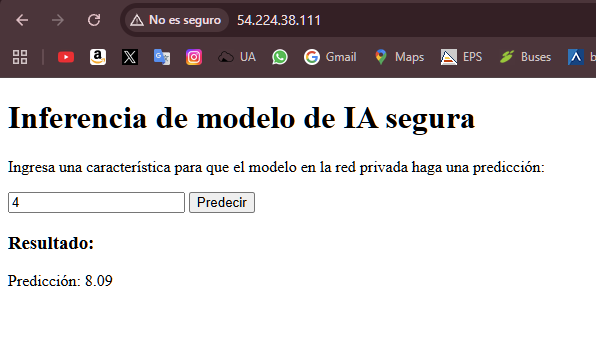
\includegraphics[width=0.8\textwidth]{prediccion_completada.png}
	\caption{predicción}
	\end{figure}

	\subsection{Prueba de despliegue 2}

<<<<<<< HEAD
	Para la aplicación de análisis de sentimiento debemos de hacer lo mismo, buscar la ip publica y conectarnos. El análisis de sentimiento según creador del modelo falla en un 10\%, yo lo he probado con estos casos y me ha funcionado bien. Seguramente el alto error de fallo se deba a que es un modelo bastante pequeño.
=======
	Para la aplicación de analisis de sentimiento debemos de hacer lo mismo, buscar la ip publica y conectarnos. El analisis de sentimiento según creador del modelo falla en un 10\%, yo lo he probado con estos casos y me ha funcionado bien. Seguramente el alto error de fallo se deba a que es un modelo bastante pequeño.
>>>>>>> 42fa237a0948d1ceb29232ede3f74fd9ab574339

	\begin{figure}[H]

	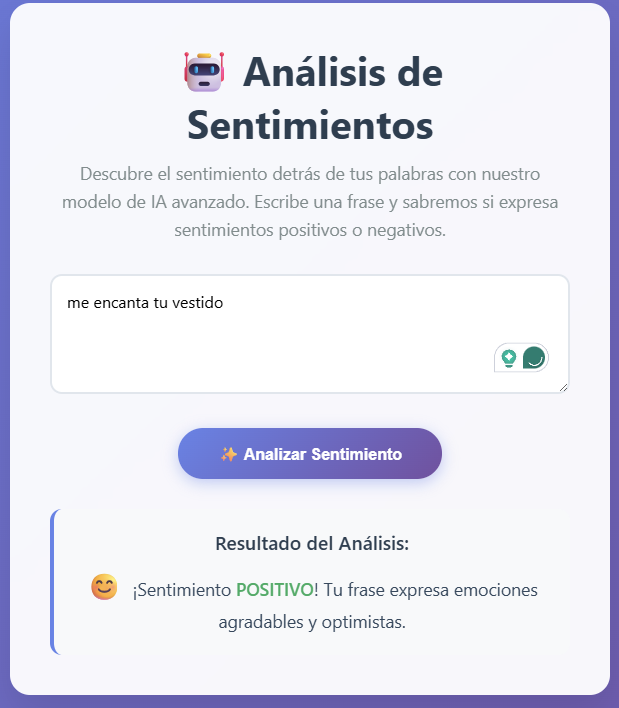
\includegraphics[width=0.5\textwidth]{prueba2.png}
	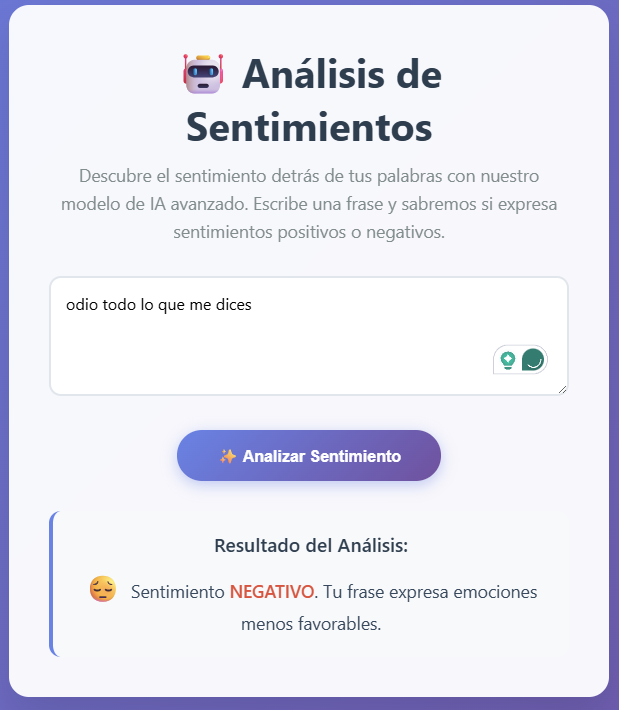
\includegraphics[width=0.5\textwidth]{prueba3.png}
	\caption{predicciones}
	\end{figure}






\end{document}
